\section{Éléments d'expérimentations sur Linear Road}\label{sec:valid:perfs:flux}
Dans cette section, nous confrontons Astronef avec le \textit{benchmark} \textit{LinearRoad}~\cite{Arasu:lrb}. L'objectif de cette confrontation n'est pas de démontrer qu'Astronef est le SGFD le plus rapide. Nous voulons par contre vérifier qu'il est possible d'obtenir des plans de requêtes aussi efficaces en écrivant directement la spécification du \textit{benchmark} en Astral.

\subsection{Le \textit{Linear Road Benchmark}}
Le \textit{Linear Road Benchmark}~\cite{Arasu:lrb} (\textit{LRB}) est un \textit{benchmark} de gestion de flux de données maintenant très répandu dans ce domaine. Le cadre d'application est de surveiller des autoroutes pour gérer les alertes d'accidents ainsi que les notifications de facturation au péage fluctuante. Une voiture ne paie le péage que si toutes ces conditions sont vérifiées : (1) il n'y avait pas d'accident dans ce segment, (2) la moyenne de vitesse des voitures du segment était inférieure à 40 et enfin (3) le nombre de voitures sur le segment était supérieur à 50. Nous avons le flux principal $P(xway, dir, seg, vid, pos, speed, \t)$ indiquant la vitesse la position (ainsi que son segment), la direction et le numéro de l'autoroute d'une voiture \textit{vid}.

Pour pouvoir calculer ces notifications en quasi temps réel\footnote{Contrainte de délai de 5 secondes maximum}, il est nécessaire de calculer aussi les vitesses moyennes des véhicules ainsi que les densités des segments. Le \textit{benchmark} permet de voir si le SGFD peut supporter la charge de $L$ autoroutes pendant trois heures. Le score du benchmark est le $L$ maximal tout en respectant les critères.

Dans cette section, nous nous intéressons avant tout à la requête de péage $T(vid,avgspeed,toll,\t)$. Son expression est grande et n'est pas présenté ici. Nous analysons ici des fragments de cette requête qui sont problématiques en terme de performances. Les autres requêtes sont des requêtes historique que nous explorons en détail avec notre cas d'application dans la section suivante.

\subsection{L'exploitation des commutativités et associativités}
L'avantage concret de l'optimisation logique à base de commutation prend tout son sens lorsqu'un langage déclaratif est utilisé. En effet, en \textit{SQL}, il est possible d'exprimer une requête Sélection-Projection-Jointure. Chaque partie est clairement défini dans les clauses du \sql{SELECT ... FROM ... WHERE}. Sa traduction en algèbre relationnelle nécessite plusieurs transformations pour obtenir une expression efficace.

A contrario, si l'expert écrit lui même sa requête en algèbre, celle-ci est déjà structurellement efficace. C'est pour cela que l'algèbre est considéré comme un langage impératif. Ainsi, nous n'avons pas pu observer de grandes optimisations avec ou sans l'optimisation logique. Toutefois, lorsqu'un langage déclaratif sera défini, cet aspect prendra de l'importance.

\subsection{Changement de segment : jointure massive et manipulation temporelle}
Dans cette partie, nous analysons la requête permettant de sélectionner les n-uplets de $P$ indiquant un changement de segment du véhicule. Cette requête peut s'écrire de cette façon : $$\RSu(P[B] \Join_{seg\neq seg2} \rho_{seg2/seg} \Pi_{xway,vid,seg} \D^{(t,i)^-}_{\t>t_0} P[xway,vid/L])$$

Plusieurs questions de performances sont à mettre en en avant :
\begin{itemize}
	\item Quel algorithme de jointure ? La taille de $P[xway,vid/L]$ risque d'être massive. Sur l'ensemble du \textit{LRB}, il existe environ 125000 valeurs différentes pour \textit{vid} pour $L=1$. La jointure par boucle imbriqué n'est pas envisageable. Le calcul d'une table de hachage est nécessaire. Nos expériences nous ont indiqué qu'à part pour des cardinalités faibles (de l'ordre de la dizaine), les jointures avec index calculé à la volée sont à privilégier même si cela implique la reconstruction de l'index à chaque évaluation.
	\item Est-ce que le mode incrémental est utilisable ? L'opérateur $\D$ permet certes de faire passer l'incrémental jusqu'à la jointure. Toutefois, la jointure n'est pas calculable facilement en incrémental car les $\delta^-$ ne sont pas nuls. De plus $P[B]$ change entièrement entre deux états. La sélection d'opérateurs statique est préférable.
	\item Dans ce cas $\IS$ et $\RSu$ ont un comportement similaire car l'intersection des états de la relation est nulle. Est-ce que l'un est privilégié par rapport à l'autre ? Comme les relations ne sont pas incrémentales, $\RSu$ a un coût linéaire tandis que $\IS$ a le coût d'une autojointure.
\end{itemize}

Voici maintenant deux optimisations logiques non triviales (mais démontrable) à cette requête.
$$\RSu(P[B] \Join_{seg\neq seg2} \rho_{seg2/seg} \Pi_{xway,vid,seg} \DS(P[xway,vid/L])[B]$$
Cette optimisation permet d'exploiter que le coût de $\DS(P[vid/L])$ est nul si l'opérateur de fenêtre partitionnées fournir une relation temporelle incrémentale (ce qui est le cas dans Astronef). Ainsi, nous obtenons deux jointures sur deux \textit{batchs} dont les cardinalités sont aux alentours de 1000~\cite{Jain:lrb}. Toutefois, le coût mémoire de $P[xway,vid/L]$ est massif car il faut tracer les 125000 identifiants. Nous notons que cette optimisation est formalisable dans Astronef.

$$\RSu(P[B] \Join_{seg\neq seg2} \rho_{seg2/seg} \Pi_{xway,vid,seg} P[T\ 30s\ 30s[$$

Nous exploitons désormais qu'un véhicule émet une données toutes les 30s. Nous exploitons aussi que notre description de fenêtre est capable de correctement traiter l'inclusion ou l'exclusion des bornes inférieures et supérieures. Nous obtenons une jointure avec une cardinalité de 30 \textit{batchs} à droite ($\sim$30000 n-uplets pour $L=1$) mais dont la table de hachage n'est calculée qu'une fois toutes les 30 secondes. À la différence, cette optimisation est plus difficile à automatiser car elle dépend des caractéristiques de $P$. Nous notons $B$ la taille d'un batch et $V$ le nombre de $vid$ différents pour une autoroute.


\begin{figure}[ht]
\centering
\begin{minipage}{0.44\textwidth}
\begin{tabular}{|c|c|c|}\bottomrule
\rowcolor{hypcolor} Stratégie & Mémoire & Calcul \\ \hline
$[./L]$ & $\O(LV)$ & $\O(LV+LB)$ \\\hline
$\DS$ & $\mathcal O(LV)$ & $\O(LB)$  \\\hline
$[T\ r\ r[$ & $\O(LB)$ & $\O(LB)$\\ \toprule
\end{tabular}
\end{minipage}
\begin{minipage}{0.55\textwidth}
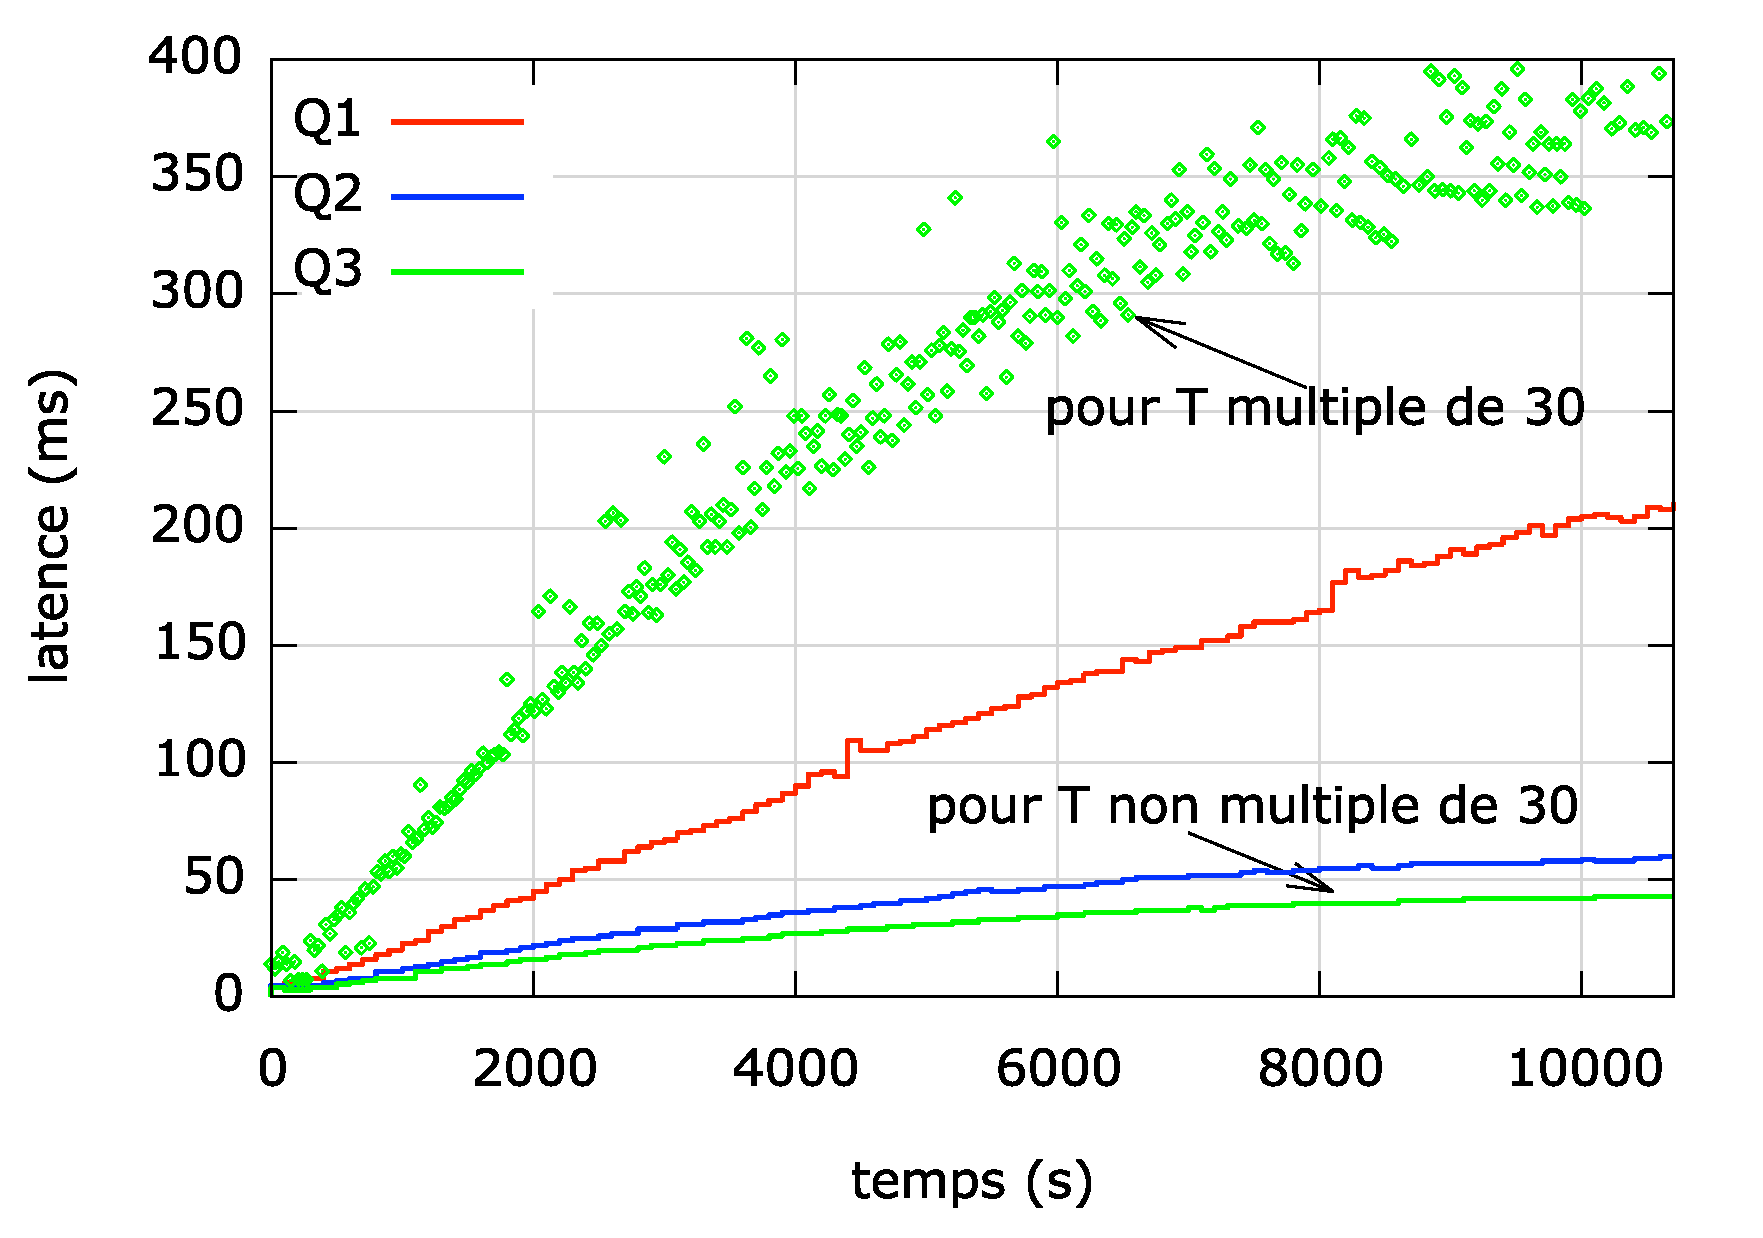
\includegraphics[width=1\textwidth]{valid-perfs-segchange}
\end{minipage}
\caption{Complexités et tracé de latence des stratégies du changement de segment}\label{fig:valid:perfs:segchange}
\end{figure}

La figure~\ref{fig:valid:perfs:segchange} trace les médianes (sur $100s$) des mesures de latences que nous obtenons. La stratégie $\DS$ évolue en fonction de la charge du benchmark alors que $[./L]$ évolue selon le nombre de voiture passé (linéaire dans notre cas). Au final, nous obtenons une latence égal à $60ms$ pour $\DS$ et $210ms$ pour $[./L]$. Enfin, la stratégie utilisant une fenêtre temporelle a une meilleure performance la plupart du temps, toutefois pour les moments où la fenêtre s'évalue ($\t\in 30\N$) alors la latence est quasiment décuplé pour passer à $350-400ms$. Néanmoins sa charge mémoire dépend uniquement de $B$.

\subsection{Calcul de vitesse d'un segment : fenêtre et agrégat}
Dans cette partie, nous analysons la requête permettant de calculer la vitesse moyenne pour un triplet \textit{(xway,dir,seg)}. Le calcul de l'agrégation telle que la spécification le présente est en trois parties comme la requête suivante le démontre :
$$\null_{\substack{xway,\\ seg,dir}}\G_{avg(tmp)}^{avgspeed}(\null_{\substack{m,xway,\\ seg,dir}}\G_{avg(tmp)}^{tmp}(\null_{\substack{vid,m,xway,\\ seg,dir}}\G_{avg(speed)}^{tmp} (e_{\lfloor T/60 \rfloor}^{m})]T\ 5min\ 1min])))$$

En supposant que nous appliquons à la lettre ce plan de requête, nous avons chaque minute : un agrégat d'environ 300000 n-uplet à appliquer, suivi de deux agrégats d'une centaine de milliers puis d'une vingtaine de millier. De plus, ce coût n'est pas amorti car l'opérateur de fenêtre est bloquant.

Pour améliorer la performance de cette requête, nous avons implémenté l'opérateur Pane~\cite{Li:pane} capable de faire des agrégations efficaces sur des fenêtres glissantes (son fonctionnement a été présenté dans la section~\ref{sec:rw:sgfd:optim:fenetres}). Le coût d'une fenêtre plus agrégation devient amorti puisque le déclenchement d'une nouvelle fenêtre produit quasiment instantanément le résultat. Toutefois, les deux autres agrégations restent à calculer avec de grandes cardinalités.

Nous avons ainsi implémenté un agrégat complexe capable de composer deux agrégats. Par exemple, l'agrégat $avg(vid/avg(speed))$ calcule la moyenne des moyennes pour chaque véhicules. La complexité en terme de mémoire et de calcul reste le même. Toutefois, il ne nécessite qu'un opérateur et lors de l'évaluation de la fenêtre, les sous-agrégats sont prêt à être calculés ce qui rend l'opération bien plus rapide. Il est de plus possible d'automatiser la réécriture de ce type d'opérations.

\begin{figure}[ht]
\centering
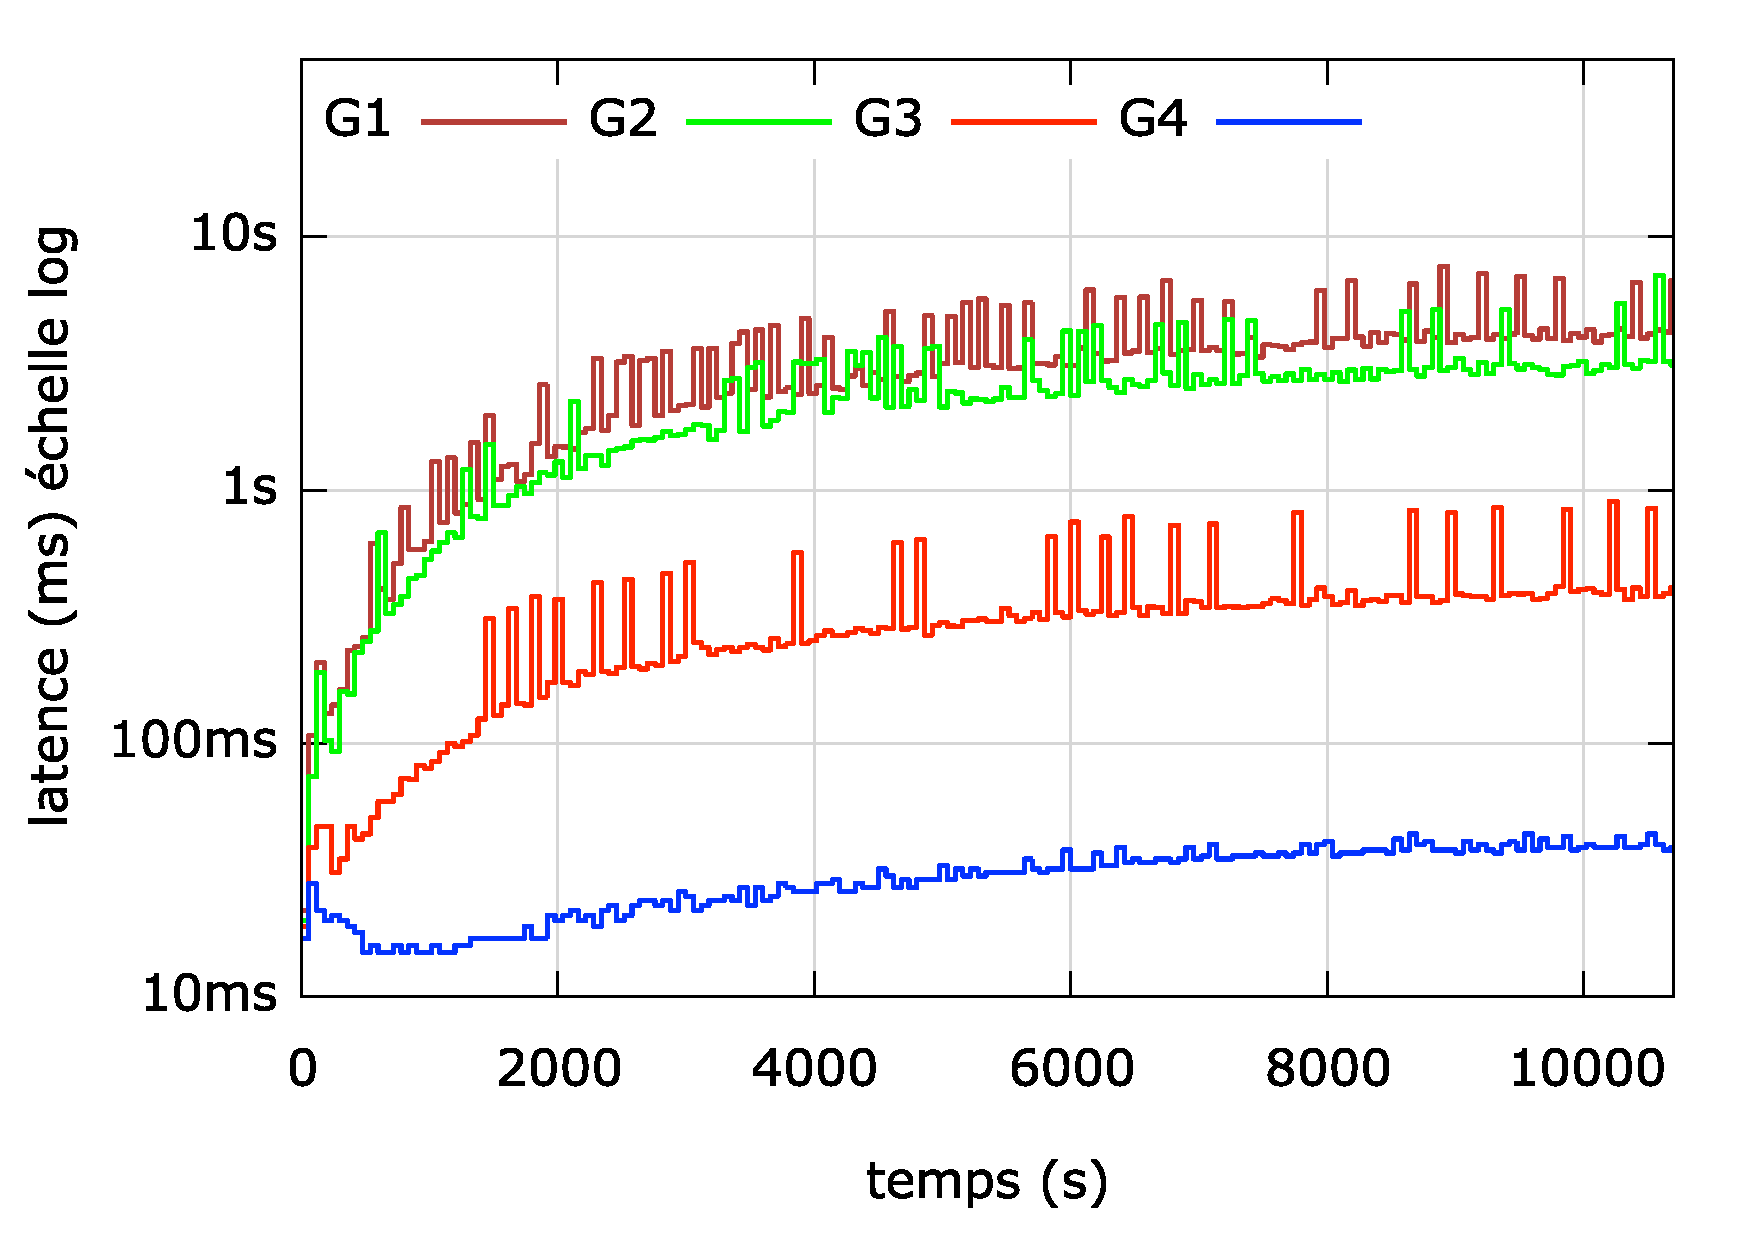
\includegraphics[width=0.6\textwidth]{valid-perfs-averagevelocity}
\caption{Tracé de la latence des stratégies pour le calcul de vitesse}\label{fig:valid:perfs:averagevelocity}
\end{figure}

La figure~\ref{fig:valid:perfs:averagevelocity} montre la latence observé sur les différentes stratégies. Nous voyons effectivement que Pane avec les deux agrégations bloquantes a des performances similaires à la fenêtre simple (gain 25\%) car peu de données sont présentes par groupes dans la première agrégation. Cependant l'agrégat complexe suit la même tendance mais avec un gain de performance de 10. Enfin, nous pouvons voir que le calcul d'un Pane simple est très efficace même sur de grandes quantités de données. De plus, il est plus stable au niveau de la mémoire car nous remarquons qu'il n'y a pas de pic de latences (dues au travail du \textit{garbage collector}).

\subsection{Allègement des structures internes}
Enfin, nous pouvons voir que nous pouvons établir des règles sur les comportements des opérateurs nous permettant de faire des économies de mémoires et de calcul en modifiant les structures internes. En effet, il existe plusieurs façon d'implémenter les relations temporelles, les flux et les séquences de n-uplets. Par exemple, il existe des structures pour les relations temporelles supportant un état, ou deux, ou $N$. De même, il existe des relations temporelles incrémentales ou non. Nous pouvons appliquer des règles permettant de décider de la meilleur structure en fonction des opérateurs.

Par exemple, dans le cadre de $\RSu(S)$. Nous pouvons indiquer : un seul état est nécessaire, l'état courant ; si la relation temporelle est incrémentale, alors il faut prévoir un entretien de l'état courant, les $\delta$ n'ont pas besoins d'être conservés. À l'inverse, $\IS$ ne nécessite que des $\delta$ ce qui évite d'entretenir l'état courant, coûteux en mémoire et en calcul.

De la même façon, nous pouvons prévoir de supprimer des vérifications de contraintes (le schéma de la séquence est respectée etc...), si l'implémentation les garanti. Sans ces optimisations, nous observons une augmentation de la latence importante (le double dans le cadre de la requête de changement de segment).
